% Part 2 - Literature study

\chapter{Video Game Theory}
\label{chapter:lit-study-game-theory}
\lhead{Chapter \ref{chapter:lit-study-game-theory}. \emph{Video Game Theory}}

This chapter looks at some previous articles on subjects related to video game theory with the goal of establishing a terminology to be used throughout the project.

\section{Pervasive Games}

In today's multitude of game genres, \emph{pervasive games} is the one that is most relevant to this project. The definition of pervasive gaming is somewhat fluid. According to Benford et al. \cite{benford2005pervasive}, \emph{"Pervasive games extend the gaming experience out into the real world"}, further stating that \emph{"The game player becomes unchained from the console and experiences a game that is interwoven with the real world and is potentially available at any place and any time"}.

Montola \cite{montola2005exploring} describes a pervasive game as \emph{"a game that has one or more salient	features that expand the contractual magic circle of play socially, spatially or temporally"}. \emph{Spatial expansion} describes the concept of expanding the play area beyond the play device itself, using a larger location such as a city or, in some cases, the whole world. \emph{Temporal expansion} refers to the distribution of game play beyond traditional play sessions. Some games define every moment to be part of the game session, while others are inactive most of the time, being played only at certain times when the game itself decides. \emph{Social expansion} means the players can go beyond those who deliberately chose to participate in the game, turning bystanders into participants through various means.

Magerkurth et al. \cite{magerkurth2005pervasive} discuss the various sub-genres of pervasive gaming, including \emph{Smart Toys}, \emph{Affective Gaming} and \emph{Augmented Tabletop Games}. The main focus of this project, however, are the \emph{Location-Aware Games} and \emph{Augmented Reality Games}.

Location-aware games determine the player's position based on technology such as GPS, WiFi, or GSM signals, or short-range proximity-sensors using RFID, Bluetooth or similar. The player can then be placed on a large-scale game board, ranging from a city block or smaller, to the entire world, and can interact with the game by physically moving.

According to Bederson \cite{bederson1995ar}, \emph{"Augmented reality uses computers to enhance the richness of the real world. It differs from virtual reality in that it doesn’t attempt to replace the real world"}. Yuen et al. \cite{yuen2011augmented} said \emph{"Augmented reality (AR) refers to a wide spectrum of technologies that project computer generated materials, such as text, images, and video, onto users’ perceptions of the real world"}. Examples of augmented reality are superimposing 3D images on a camera view or playing audio based on the user's location and movement.

Kiefer et al. \cite{kiefer2006systematically} explored the design space of location-aware or location-based games, identifying three \emph{game design dimensions}, positing that new games can be created by choosing values for each of the three dimensions, or by taking an existing game and changing one of the dimensions. The first of the three dimensions is the dimension of \emph{game environmental embedding}, which \emph{"deals with the way the game world is embedded in the player’s environment"}, distinguishing between \emph{pure location-based games}, \emph{mixed reality location-based games} and \emph{augmented reality location-based games}.

They define a location-based game as \emph{"a game which is supported by localization technology and integrates the position of (one or several) players as main game element into its rules"}, focusing on the requirement that the game rules rely on the localization technology. Mixed reality location-based games refer to games where virtual objects affect the physical game space, but exist only in the virtual layer and cannot be perceived by the players in their physical location. Augmented reality location-based games on the other hand allow players to players to perceive the virtual game elements \emph{"from a first-person perspective"}.

The second dimension is the \emph{game conceptual dimension}, which refers to the concept and goals of the game, on a more specific level than the established game genres. They define four types game concepts for location-based games: \emph{Chase game}, \emph{Item hunt game}, \emph{Puzzle game} and \emph{Strategy game}. A chase game is a game were a player's physical speed is central in the pursuit of victory, and are typically technology-supported variants of the classic playground game of \emph{Tag}. Item hunt games involves the search for items hidden throughout the game board, while puzzle games have you solve one or more puzzles toward some ultimate goal. Strategy games require the player to plan their moves to win.

The third and final dimension is the \emph{spatial and temporal dimension}, where games can be either spatially continuous or discrete, and either temporally continuous or discrete. Spatially discrete (sd) games have game events take place only in specific locations, while spatially continuous (sc) games can progress the game anywhere. Similarly, temporally discrete (td) games allow movement in the game only at given moments, while temporally continuous (tc) games allow game progress and events at any time. They identified games with the \emph{sdtd}, \emph{sdtc} and \emph{sctc} combinations, but no \emph{sctd} games.

\todo{References throughout project}

\section{Player Types}
\label{sec:player-types}

Player types are a way of categorizing players on various axes with the goal of creating an enjoyable game experience for the target audience. Identifying player types can also be important for developers of games whose business model is to sell in-game items rather than retail sale of the game itself, as Hamari \& Tuunanen \cite{hamari2014playertypes} discussed in their 2014 meta-synthesis on the subject. The design of such items is largely based on the potential customers, and what type of items will be sold will depend on who are going to play the game and what their motivations are.

There are countless studies on different player types, and Hamari \& Tuunanen \cite{hamari2014playertypes} compared the different ways previous researchers have segmented players to create their typologies, using primarily behavioral and psychographic segmentation, but sometimes also geographic or demographic segmentation.

They found that a common division was that of \emph{hardcore} and \emph{casual} players, but found this to be a too simplistic solution. Hardcore players were sometimes described to be more dedicated in all areas of the games, playing for longer sessions, more often and being more invested. However, they found that all these aspects and more were better treated separately, creating multiple scales used to define more than just two types of players.

Kallio et al. \cite{kallio2011gamermentalities} used a model consisting of the scales of \emph{Intensity} and \emph{Sociability}, along with a \emph{Games} component to define three different groups of gamer mentalities. The components of the model can be seen in Figure \ref{fig:kallio-gamer-mentalities-model}, as presented in their paper, and the three groups of mentalities they define using this model are \emph{Social mentality profiles}, \emph{Casual mentality profiles} and \emph{Commited mentality profiles}.

\begin{figure}[h]
	\centering
	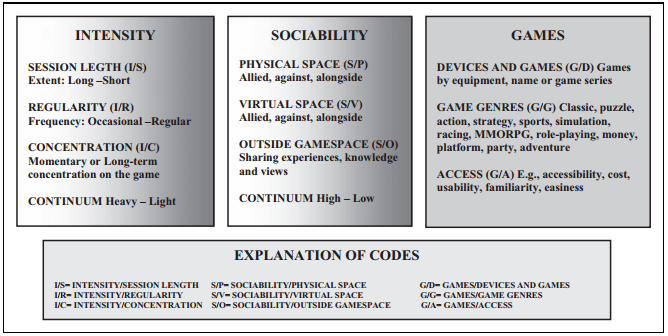
\includegraphics[width=\textwidth]{Figures/kallio-gaming-mentalities-model}
	\caption{The three components of gaming mentalities, as seen in Kallio et al. \cite{kallio2011gamermentalities}}
	\label{fig:kallio-gamer-mentalities-model}
\end{figure}

The social mentality profiles identified by Kallio et al. are of \emph{"quite light"} intensity, very high sociability and their choice in games focus on access to the games. The casual mentality profiles have variable intensity, low sociability and their choice in games focuses primarily on the device and access. The committed mentality profiles have \emph{"heavy"} intensity, high sociability and their choice in games focuses primarily on the genre. Each of the groups of profiles consist of three profiles with different, although similar, values for the various metrics defined in the model. \advice{Is this paragraph (or even source) really of any use here?}

Hamari \& Tuunanen \cite{hamari2014playertypes} used this and other papers to identify a total of five \emph{"key dimensions pertaining to motivations of play/orientation of the player"}: \emph{Achievement}, \emph{Exploration}, \emph{Sociability}, \emph{Domination} and \emph{Immersion}.

In this project, we will use the five archetypal player types \emph{Achieving}, \emph{Exploring}, \emph{Socializing}, \emph{Dominating} and \emph{Immersing}, where each of them is \emph{more concerned with} their respective dimension of the game than the four others, rather than \emph{entirely focused on} only that aspect. That is, for a \emph{Socializing} player, the social aspect of the game is more important than any other aspect, but they may still have varying interest in the other four dimensions.

\todo{Reference these types other places in the report}

\section{Motivation in Gaming}
\label{sec:motivation-in-gaming}

When considering motivation, we typically distinguish between \emph{intrinsic} and \emph{extrinsic} motivation. \emph{Extrinsic motivation} is motivation from outside sources such as the promise of receiving rewards for successful completion of a task, or punishment should one fail to complete the task. \emph{Intrinsic motivation} on the other hand refers to motivation coming from within, where performing a task is in itself personally rewarding, either because it is fun, exciting, enjoyably challenging or a variety of other positive emotions.

Malone \cite{malone1981toward} proposes challenge, fantasy and curiosity as the primary factors of intrinsic motivation in gaming. Looking back at the player types established in Section \ref{sec:player-types}, the Achieving and Dominating players have challenge as their primary intrinsic motivator, while the Immersing player is motivated by fantasy and the Exploring player is motivated by curiosity. The Socializing player's main source of motivation is not related to the game itself.

While some studies suggest that extrinsic motivation can conflict with and undermine intrinsic motivation (see for example Benabou \& Tirole \cite{benabou2003intrinsic}, Lepper \& Henderlong \cite{lepper2000motivation}), extrinsic rewards are common in video games. By progressing or performing difficult tasks in games, players unlock new types of items or characters, receive powerful items or abilities, in-game currency, cosmetic modifications to their avatar, recognition from other players from being placed in a hall of fame or leader board of some kind, or any number of other rewards. For some, these rewards do indeed remove the fun - the intrinsic motivation - from the game, turning it into a chase for the next reward. For others, however, these rewards help bring back the fun they were no longer able to find, enjoying the game more when being rewarded.

In a market with hundreds of thousands of games and players with short attention spans, however, extrinsic rewards for small feats has become common. To keep players active, they are awarded for doing a minimal amount of effort every day through daily reward systems, often of the form \emph{First X of the day}. For some developers, this is the final step for the game: a last resort to keep players playing their game. For others, it's a means to bridge the gap until they can introduce new features.


% Chapter - Current state of physical and mental health in society (western world?)
\chapter{Modern Society and Health}
\label{chapter:lit-study-modern-health}
\lhead{Chapter \ref{chapter:lit-study-modern-health}. \emph{Modern Society and Health}}

\section{Physical Activity}
\label{sec:lit-study-physical-activity}

\todo{About increasingly sedentery lifestyles in modern society, the effects of just moving a little every day etc}

\section{Mental Health}
\label{sec:lit-study-mental-health}

\todo{About the effects of gaming (having fun, accomplishing goals), being social, and exercising}


\chapter{Similar Games}
\label{chapter:lit-study-game-types}
\lhead{Chapter \ref{chapter:lit-study-game-types}. \emph{Game Types}}

\section{Location-Based, Augmented Reality, and Pervasive Games}
\label{sec:prestudy-ar-location-pervasive-games}

\section{Exergames}

\todo{Zombies Run, Stolpejakten, Munzee, Run an Empire}

\section{Mobile Games}
\label{sec:mobile-games}

\todo{Talk about typical mobile games, microtransactions etc}

\section{Similar Games}

\todo{Ingress, Geocaching, ++}


% Chapter - More about Pokémon and Pokémon GO
\chapter{Pokémon GO}
\label{chapter:lit-study-pokemon-go}
\lhead{Chapter \ref{chapter:lit-study-pokemon-go}. \emph{Pokémon GO}}

\section{Pokémon Franchise}
\todo{Short introduction to the Pokémon franchise, some terms and the different games?}

\section{Pokémon GO In-Depth}
\label{sec:pokemon-go-in-depth}
\todo{Tech choices for GO and differences from "main" games}

\section{Pokémon GO and Video Game Theory}
\label{sec:pokemon-go-theory}
\todo{Elaborate on Pokémon GO with the theory from this chapter.}
